\section{Tập dữ liệu, phân tích đặc trưng và pipeline tiền xử lý}

\subsection{Nguồn dữ liệu và cấu trúc ngữ nghĩa ban đầu}

Bộ dữ liệu nền của đề tài được lấy từ Kaggle, cụ thể là dataset \texttt{Used Phones \& Tablets Pricing Dataset} của tác giả \texttt{ahsan81}. Theo mô tả nguồn, dataset này được xây dựng cho các bài toán phân tích giá và dự đoán giá của thiết bị cầm tay đã qua sử dụng; tập dữ liệu gốc có 3.454 bản ghi và 15 trường dữ liệu. Ở góc nhìn nghiệp vụ, mỗi bản ghi biểu diễn một thiết bị đã qua sử dụng cùng với thông tin cấu hình, vòng đời sử dụng và mặt bằng giá tương ứng.

Để mô tả ngắn gọn bộ dữ liệu gốc, có thể tóm tắt như sau:

\begin{center}
\begin{tabular}{|l|l|}
\hline
\textbf{Thuộc tính} & \textbf{Mô tả} \\
\hline
Nguồn dữ liệu & Kaggle -- \texttt{Used Phones \& Tablets Pricing Dataset} \\
\hline
Đơn vị quan sát & Một thiết bị cầm tay đã qua sử dụng \\
\hline
Quy mô dữ liệu gốc & 3.454 bản ghi, 15 trường \\
\hline
Mục tiêu sử dụng & Phân tích giá và xây dựng mô hình dự đoán giá \\
\hline
Dạng bài toán & Hồi quy trên dữ liệu bảng \\
\hline
\end{tabular}
\end{center}

Ở mức trường dữ liệu, bộ gốc bao gồm các cột: \texttt{device\_brand}, \texttt{os}, \texttt{screen\_size}, \texttt{4g}, \texttt{5g}, \texttt{rear\_camera\_mp}, \texttt{front\_camera\_mp}, \texttt{internal\_memory}, \texttt{ram}, \texttt{battery}, \texttt{weight}, \texttt{release\_year}, \texttt{days\_used}, \texttt{normalized\_used\_price} và \texttt{normalized\_new\_price}. Cấu trúc này cho thấy dataset không chỉ chứa thông số kỹ thuật của thiết bị, mà còn chứa trực tiếp hai biến giá ở dạng log-price để phục vụ các bài toán hồi quy.

Để phục vụ hệ thống hiện tại, dữ liệu gốc được đưa về một schema vận hành thống nhất. Tập dữ liệu cục bộ đang được sử dụng tại \path{Mobile-Phone-Price-Prediction/app/data/sample_phone_data.csv} có 3.454 bản ghi và 13 cột, tức đã lược bỏ hai cột kết nối \texttt{4g} và \texttt{5g}. Việc thu gọn này phản ánh đúng định hướng của pipeline hiện hành: chỉ giữ các biến đang thực sự đi vào huấn luyện và suy luận, từ đó làm schema ổn định hơn cho cả nhập liệu, train và runtime.
Từ góc nhìn ngữ nghĩa, các trường của dữ liệu có thể được tổ chức thành ba nhóm lớn:
\begin{itemize}
    \item \textbf{Nhóm nhận diện và cấu hình:} \texttt{device\_brand}, \texttt{os}, \texttt{screen\_size}, \texttt{rear\_camera\_mp}, \texttt{front\_camera\_mp}, \texttt{internal\_memory}, \texttt{ram}, \texttt{battery}, \texttt{weight}.
    \item \textbf{Nhóm vòng đời sử dụng:} \texttt{release\_year}, \texttt{days\_used}.
    \item \textbf{Nhóm giá trị thị trường:} \texttt{normalized\_used\_price}, \texttt{normalized\_new\_price}.
\end{itemize}

\subsection{Chuẩn hóa dữ liệu, xây dựng đặc trưng}

Khi nhập bản ghi thủ công hoặc import CSV, dữ liệu đều được đưa qua bước chuẩn hóa schema để bảo đảm đủ cột, đúng tên trường và đúng cách biểu diễn giá trị mục tiêu. Các bước bao gồm: 
\begin{enumerate}[label=\arabic*.]
    \item kiểm tra dữ liệu đầu vào có khớp \texttt{RAW\_SCHEMA} hay không;
    \item chuẩn hóa kiểu dữ liệu của các cột số như \texttt{screen\_size}, \texttt{ram}, \texttt{battery}, \texttt{release\_year} và \texttt{days\_used};
    \item chuyển giá thô về dạng \texttt{normalized\_used\_price} và \texttt{normalized\_new\_price} nếu dữ liệu nhập ở dạng giá gốc;
    \item ánh xạ dữ liệu nguồn sang tập đặc trưng huấn luyện thống nhất;
    \item tách giữa tập đặc trưng đầy đủ và tập đặc trưng mặc định để phục vụ train theo cấu hình chuẩn hoặc train thử nghiệm.
\end{enumerate}

Sau bước chuẩn hóa, phần feature engineering được thực hiện để tạo ma trận huấn luyện. Trong bước này, dữ liệu gốc được ánh xạ về tập đặc trưng phù hợp với mô hình Random Forest, đồng thời phân tách giữa tập đặc trưng đầy đủ và tập đặc trưng mặc định. Tập đầy đủ cho phép mở rộng khi cần thử nghiệm, còn tập mặc định giữ vai trò cấu hình ổn định cho các lần huấn luyện thông thường.

\subsection{Đặc điểm thống kê của dữ liệu, EDA và chiến lược tăng cường mẫu}

Trên tập dữ liệu cục bộ hiện tại, phân bố thương hiệu không đồng đều. Năm nhóm xuất hiện nhiều nhất lần lượt là \texttt{Others} (502 bản ghi), \texttt{Samsung} (341), \texttt{Huawei} (251), \texttt{LG} (201) và \texttt{Lenovo} (171). Điều đó cho thấy dữ liệu nghiêng mạnh hơn về một số nhóm phổ biến, kéo theo nguy cơ mô hình học tốt hơn ở các nhóm đông mẫu nhưng kém ổn định hơn ở các nhóm hiếm.

Ngoài mất cân bằng theo thương hiệu, dữ liệu hiện hành cũng còn giá trị thiếu ở một số cột cấu hình. Đáng chú ý nhất là \texttt{rear\_camera\_mp} thiếu 179 giá trị; các cột như \texttt{battery}, \texttt{weight}, \texttt{internal\_memory} và \texttt{ram} cũng có thiếu hụt ở mức nhỏ hơn. Điều này cho thấy dataset dùng trong hệ thống không thể được xem là đầu vào đã hoàn toàn sạch, mà cần đi qua bước chuẩn hóa và kiểm tra schema trước khi huấn luyện.

Trạng thái của tập dữ liệu đang dùng có thể tóm tắt ngắn gọn như sau:

\begin{center}
\begin{tabular}{|l|l|}
\hline
\textbf{Khía cạnh} & \textbf{Quan sát} \\
\hline
Phân bố thương hiệu & không đồng đều, nghiêng về một số nhóm phổ biến \\
\hline
Giá trị thiếu & xuất hiện ở một số cột cấu hình phần cứng \\
\hline
Biến giá mục tiêu & đã có sẵn ở dạng log-price \\
\hline
Hàm ý cho pipeline & cần chuẩn hóa dữ liệu và kiểm soát đại diện mẫu \\
\hline
\end{tabular}
\end{center}

Nhằm phục vụ quá trình phân tích dữ liệu, các biểu đồ trực quan hóa dữ liệu được tổ chức thành ba lớp phân tích chính, trong đó mỗi lớp gắn với một mục tiêu đọc dữ liệu cụ thể:
\begin{itemize}
    \item \textbf{Phân phối đơn biến số:} trong nhóm này, \textbf{box plot} hỗ trợ phát hiện ngoại lệ và các khoảng giá trị bất thường, còn \textbf{distribution plot} kết hợp KDE giúp nhận diện độ lệch phân phối, vùng mật độ tập trung và khả năng tồn tại nhiều cụm giá trị.
    \begin{figure}[H]
        \centering
        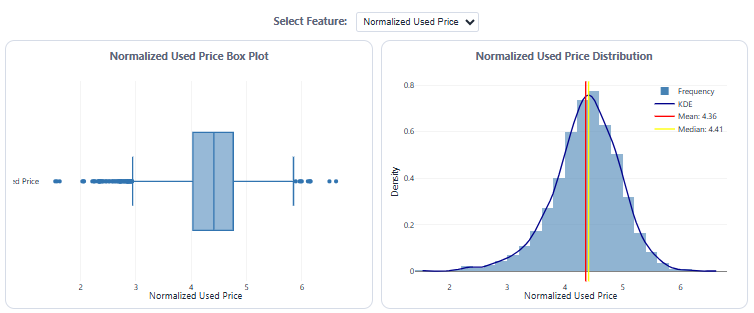
\includegraphics[width=0.88\textwidth]{graphics/data_visualize/data_distributions.png}
        \caption{Biểu đồ phân phối đơn biến số}
    \end{figure}
    \item \textbf{Quan hệ giữa các biến:} correlation matrix trên toàn bộ các cột số và cho phép dựng scatter plot giữa hai biến bất kỳ, mặc định theo hướng một đặc trưng so với \texttt{normalized\_used\_price}. Ở đây, \textbf{correlation matrix} được dùng để nhận diện các cặp biến có quan hệ mạnh nhằm hỗ trợ chọn đặc trưng, trong khi \textbf{scatter plot} giúp kiểm tra trực quan mức độ liên hệ giữa giá máy cũ với các biến.
    \begin{figure}[H]
        \centering
        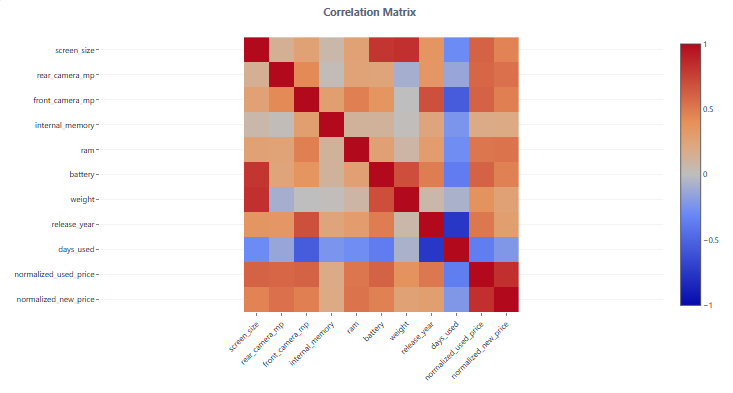
\includegraphics[width=0.88\textwidth]{graphics/data_visualize/feature_relationships.png}
        \caption{Biểu đồ thể hiện quan hệ giữa các đặc trưng.}
    \end{figure}
    \item \textbf{Phân bố theo nhóm:} các đồ thị tần suất của các biến dùng để đọc cấu trúc mẫu của dữ liệu. Nhóm biểu đồ này đặc biệt hữu ích trong việc đánh giá mức độ mất cân bằng dữ liệu như giữa các thương hiệu, hệ điều hành và các mức cấu hình phổ biến.
    \begin{figure}[H]
        \centering
        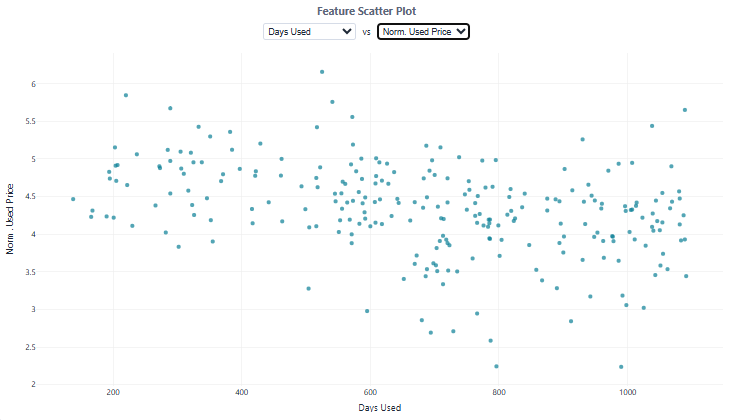
\includegraphics[width=0.82\textwidth]{graphics/data_visualize/feature_scatter_plot.png}
        \caption{Biểu đồ phân bố mẫu và cấu trúc dữ liệu.}
    \end{figure}
\end{itemize}

Như vậy, các biểu đồ trực quan hóa này sẽ là công cụ hỗ trợ data scientist đưa ra quyết định về làm sạch dữ liệu và xử lý ngoại lệ, lựa chọn hoặc ưu tiên đặc trưng cho mô hình, cũng như xác định có cần tăng cường dữ liệu để bù mất cân bằng mẫu hay không.

Từ đặc điểm đó, phần augmentation được thêm vào như một bước chủ động điều chỉnh phân bố dữ liệu. Cơ chế tăng cường mẫu trong dự án tập trung vào việc sinh dữ liệu iPhone tổng hợp với nhiều hồ sơ phân phối khác nhau. Thay vì sinh ngẫu nhiên theo một cách duy nhất, dữ liệu tổng hợp được tổ chức theo nhiều profile để có thể điều chỉnh mức độ tập trung vào máy đời mới, mức phân bố cân bằng hơn hoặc mức thiên về một nhóm cấu hình cụ thể. Việc giữ nhiều profile như vậy giúp augmentation không trở thành một thao tác cứng, mà là một phần của chiến lược dữ liệu có thể thay đổi theo mục tiêu huấn luyện.

Về mặt thực tiễn, augmentation không nhằm thay thế dữ liệu thật mà nhằm lấp bớt khoảng trống đại diện của một số nhóm thiết bị. Toàn bộ phần này được đặt trực tiếp vào ứng dụng để data scientist có thể điều chỉnh dữ liệu ngay trong luồng vận hành.


Sau khi dữ liệu đã được dựng thành ma trận huấn luyện, pipeline thực hiện chia train-test theo tỷ lệ 80/20. Cách chia này được dùng để tạo ra một mặt bằng đánh giá thống nhất giữa các version mô hình. Dù đây là cấu hình cơ bản, nó vẫn đủ để đối chiếu nhanh các lần huấn luyện trong phạm vi ứng dụng cục bộ.

Xét trên toàn bộ quá trình chuẩn bị dữ liệu, pipeline hiện tại được xây dựng quanh ba yêu cầu: dữ liệu phải có schema thống nhất, phải có khả năng tăng cường khi thiếu đại diện và phải giữ được tính nhất quán khi đi từ nhập liệu đến huấn luyện rồi sang suy luận. Ba yêu cầu này tạo thành phần xương sống của toàn bộ vòng đời dữ liệu trong ứng dụng.
